%%%%%% DON'T MODIFY STARTING HERE
\newpage
\section*{3. End Effectors}

For this section, you may reference the template code or the \href{https://document.wlkata.com/?doc=/wlkata-mirobot-resources-for-education/python-sdk/#header-step-8npsc}{documentation}.
You will perform the same task using 3 different end effectors.
%
\begin{figure}[h!]
    \centering
    \begin{subfigure}[b]{0.27\textwidth}
        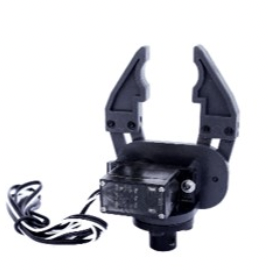
\includegraphics[width=2cm]{image/gripper.png}
        \caption*{Gripper}
    \end{subfigure}
    \hfill
    \begin{subfigure}[b]{0.27\textwidth}
        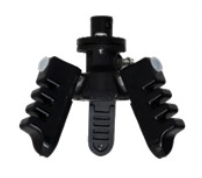
\includegraphics[width=2cm]{image/3finger.png}
        \caption*{Flexible Claw}
    \end{subfigure}
    \hfill
    \begin{subfigure}[b]{0.27\textwidth}
    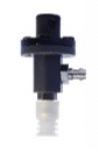
\includegraphics[width=1.2cm]{image/suction cup.png}
    \caption*{Suction Cup}
    \end{subfigure}
    \caption*{Types of end effectors.}
\end{figure}

\paragraph{3A.} Change end effectors. Attach a picture of each after successfully attaching each end effector.
\begin{enumerate} %[(i)]
    \item Power off the robot
    \item For the gripper, connect it to the correct port on the Multifunctional Extender Box (MEB). For the claw and suction cup, connect the pneumatic pump to the MEB.
    Make sure to connect the pump to the gripper as needed.
\begin{figure}[H]
  \centering
  \vspace*{-0.0 in}
  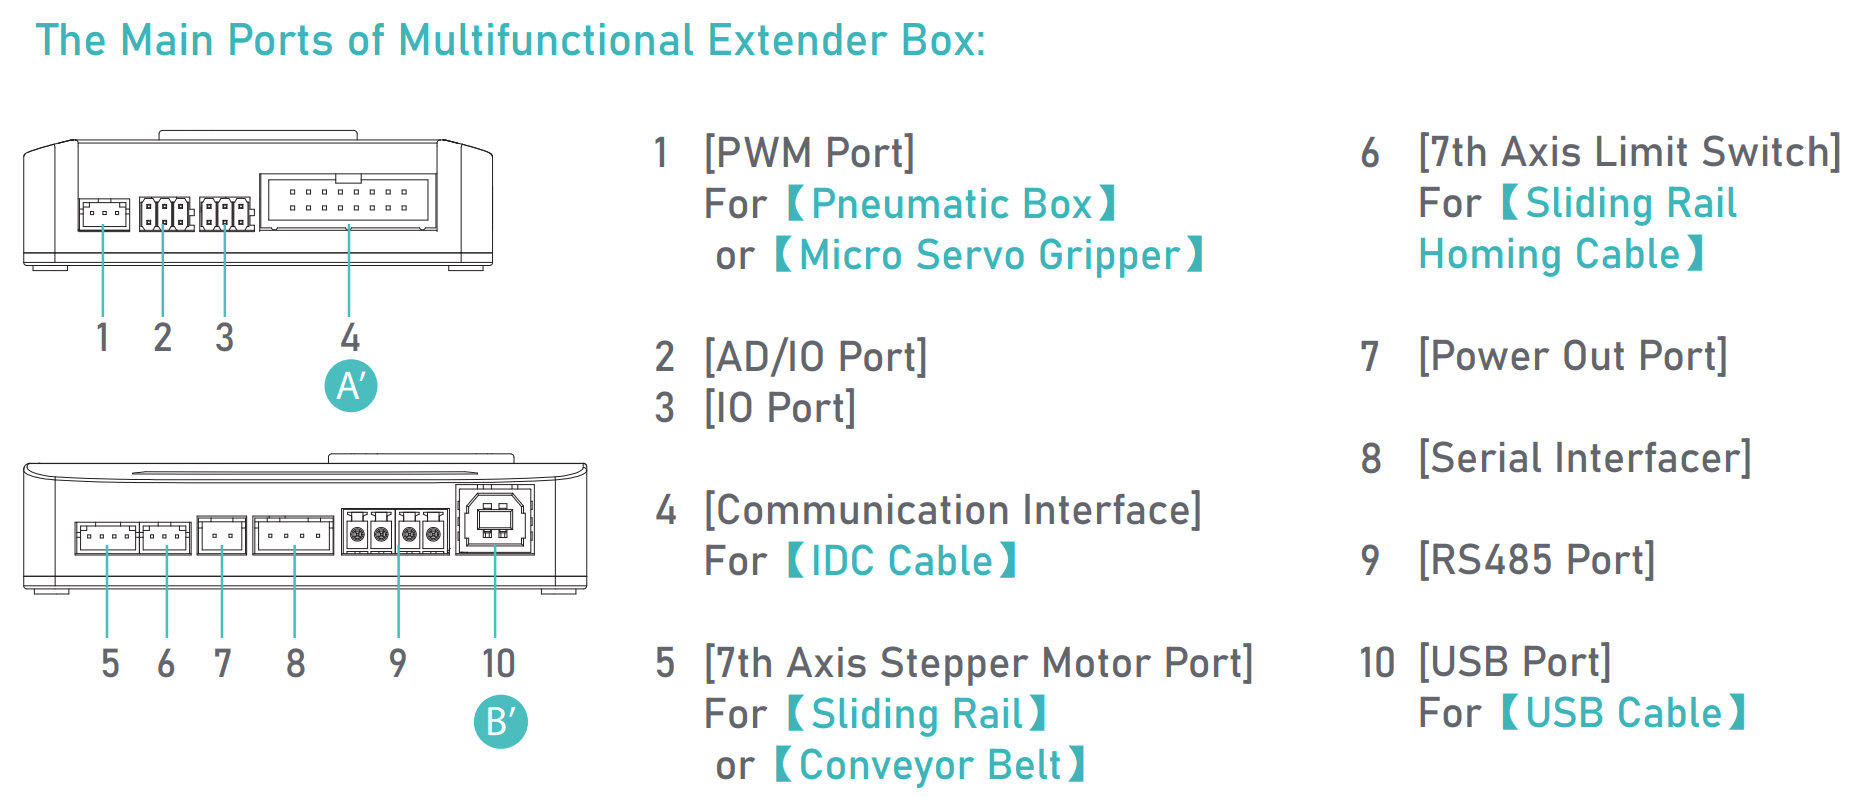
\includegraphics[width=10cm]{image/endeffectors.png}
  \caption*{Use port 1 to connect the end effectors}
  \end{figure}
    \item Connect the MEB to the robot.
    \item Screw on the end effector (an Allen wrench is the the tool box).
    Be careful to connect all wires before screwing on the end effector.
    \begin{figure}[H]
   \centering
    \vspace*{-0.0 in}
    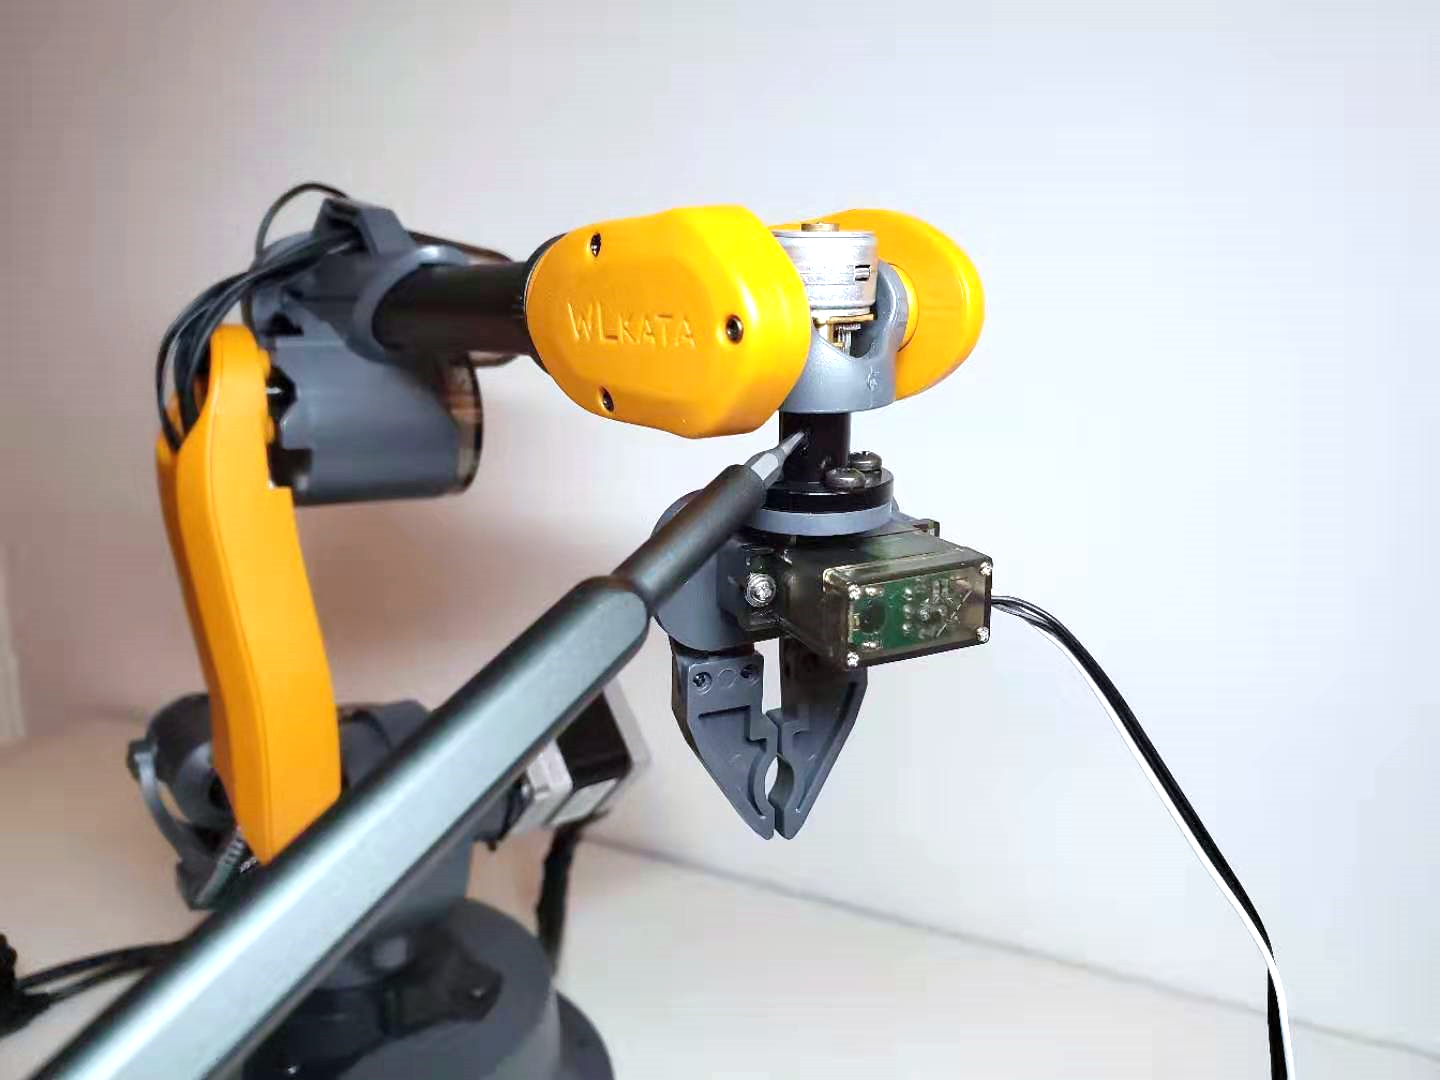
\includegraphics[width=10cm]{image/screwingendeffector.png}
    \caption*{How to screw on the end effector. Use the Allen wrench in the toolbox.}
\end{figure}
\end{enumerate}

\paragraph{3B.} Use the gripper (2 finger) to grab any toy block from the table. Submit photo result of the robot successfully lifting a block in the space provided.
    \begin{enumerate}
        \item Complete the task using the studio software
        \item Complete the task using Python API
        \begin{itemize}
        \item \texttt{from wlkata\_mirobot import WlkataMirobotTool}
        \item \texttt{arm.set\_tool\_type(WlkataMirobotTool.GRIPPER)}
        \item \texttt{arm.gripper\_open()}
        \item \texttt{arm.gripper\_close()}
        \item \texttt{arm.set\_gripper\_spacing(spacing\_mm)}
        \end{itemize}
    \end{enumerate}
    
\paragraph{3C.} Use the flexible claw (3 finger soft gripper) to grab any block from the table. Submit photo result of the robot successfully lifting a block in the space provided.

    
    \begin{enumerate}
        \item Complete the task using the studio software
        \item Complete the task using Python API
        \begin{itemize}
        \item For flexible claws, air pump suction represents opening and blowing represents closing.
        \item \texttt{arm.set\_tool\_type(WlkataMirobotTool.FLEXIBLE\_CLAW)}
        \item \texttt{arm.pump\_suction()}
        \item \texttt{arm.pump\_blowing()}
        \end{itemize}
    \end{enumerate}

\paragraph{3D.} Use the suction cup to grab any block from the table. Submit photo result of the robot successfully lifting a block in the space provided.

    \begin{enumerate}
        \item Complete the task using the studio software
        \item Complete the task using Python API
        \begin{itemize}
        \item \texttt{arm.set\_tool\_type(WlkataMirobotTool.FLEXIBLE\_CLAW)}
        \item \texttt{arm.pump\_suction()}
        \item \texttt{arm.pump\_blowing()}
        \end{itemize}
    \end{enumerate}
     \begin{figure}[H]
   \centering
    \vspace*{-0.0 in}
    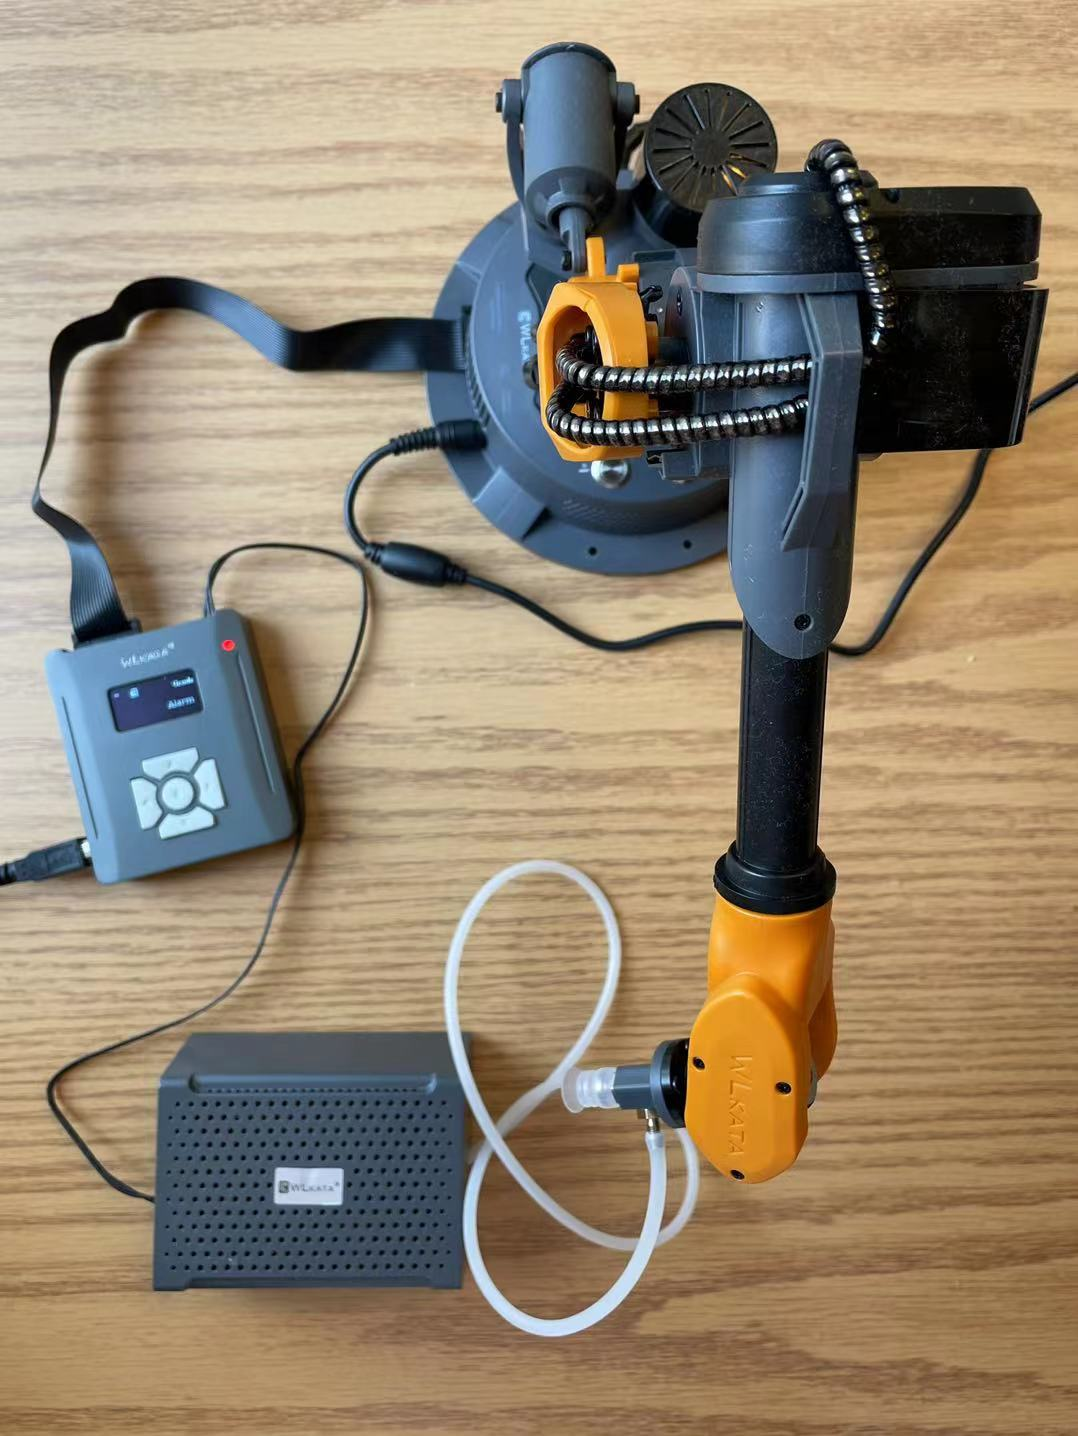
\includegraphics[width=10cm]{image/vacuumsetup.jpg}
    \caption*{Image showing how to use the pneumatic pump.}
\end{figure}
%%%%%% DON'T MODIFY UNTIL HERE

\newpage
\paragraph{Answers.}
Please do not exceed the height provided for each answer image.
%%%%%% YOU ANSWER STARTS HERE

% NOTE: MAKE SURE YOU DON'T CHANGE THE HEIGHT OF IMAGES
% NOTE: MAKE SURE TO REMOVE THE 'draft' OPTION FOR includegraphics BELOW. OTHERWISE, YOU WILL NOT SEE YOUR IMAGES.

\paragraph{3A. Change End Effectors}
%
\begin{figure}[h!]
    \centering
    \begin{subfigure}[b]{0.3\textwidth}
        \includegraphics[draft,height=2.5in]{YOUR\_ANSWER.png}
         \caption*{Mirobot with Gripper.}
     \end{subfigure}
     %
     \hfill
     %
     \begin{subfigure}[b]{0.3\textwidth}
        \includegraphics[draft,height=2.5in]{YOUR\_ANSWER.png}
         \caption*{Mirobot with Flexible Claw.}
     \end{subfigure}
     %
     \hfill
     %
     \begin{subfigure}[b]{0.3\textwidth}
        \includegraphics[draft,height=2.5in]{YOUR\_ANSWER.png}
         \caption*{Mirobot with Suction Cup.}
     \end{subfigure}     
    \caption*{Answer for 3A.}
\end{figure}
%
\begin{minted}{python}
    var = 'YOU CODE GOES HERE'
\end{minted}

\newpage
\paragraph{3B. Using Gripper.}
\begin{figure}
    \centering
    \begin{subfigure}[b]{0.3\textwidth}
        \includegraphics[draft,height=2.5in]{YOUR\_ANSWER.png}
         \caption*{Gripper lifting a block (WLKATA Studio).}
     \end{subfigure}
     %
     \hfill
     %
     \begin{subfigure}[b]{0.3\textwidth}
        \includegraphics[draft,height=2.5in]{YOUR\_ANSWER.png}
         \caption*{Gripper lifting a block (Python).}
     \end{subfigure}
    \caption*{Answer for 3B.}
\end{figure}
%
\begin{minted}{python}
    var = 'YOU CODE GOES HERE'
\end{minted}


\newpage
\paragraph{3C. Using Flexible Claw.}
\begin{figure}
    \centering
    \begin{subfigure}[b]{0.3\textwidth}
        \includegraphics[draft,height=2.5in]{YOUR\_ANSWER.png}
         \caption*{Flexible Claw lifting a block (WLKATA Studio).}
     \end{subfigure}
     %
     \hfill
     %
     \begin{subfigure}[b]{0.3\textwidth}
        \includegraphics[draft,height=2.5in]{YOUR\_ANSWER.png}
         \caption*{Flexible Claw lifting a block (Python).}
     \end{subfigure}
    \caption*{Answer for 3C.}
\end{figure}
%
\begin{minted}{python}
    var = 'YOU CODE GOES HERE'
\end{minted}


\newpage
\paragraph{3D. Using Suction Cup.}
\begin{figure}
    \centering
    \begin{subfigure}[b]{0.3\textwidth}
        \includegraphics[draft,height=2.5in]{YOUR\_ANSWER.png}
         \caption*{Suction Cup lifting a block (WLKATA Studio).}
     \end{subfigure}
     %
     \hfill
     %
     \begin{subfigure}[b]{0.3\textwidth}
        \includegraphics[draft,height=2.5in]{YOUR\_ANSWER.png}
         \caption*{Suction Cup lifting a block (Python).}
     \end{subfigure}
    \caption*{Answer for 3D.}
\end{figure}
%
\begin{minted}{python}
    var = 'YOU CODE GOES HERE'
\end{minted}


\newpage
\paragraph{Additional Space.}
Please do not exceed this page for this question.
%%%%%% YOU ANSWER ENDS HERE
